\documentclass[../main.tex]{subfiles}
\begin{document}
    \subsection{Zeeman Effekt}
        Der erste Teil der Versuchsreihe beschäftigt sich mit dem transversalen Aufbau. Gemäß der Anleitung wird vor dem Start der Messreihen die Justage der Geräte vorgenommen. Hierzu wird unter anderem die Cd Lampe mittig zwischen den Polschuhen des Magneten platziert und das Interferenzabbild im Fernrohr durch optische Justage optimiert. Als erste Messung wird durch Stromeinstellung am Elektromagneten eine äquidistante Aufspaltung der Cd Linien erzeugt und per Hall Sonde die herrschende Flussdichte im Magnetfeld gemessen. Dieser Messablauf wird zur statistischen Mittelung mehrfach wiederholt. Eine qualitative Beobachtung der Auswirkung eines Polarisationsfilters und dessen Drehwinkel auf das Interferenzbild wird ebenfalls nach Abschluss der ersten Messreihe durchgeführt.

        Im longitudinalen Aufbau wird der Elektromagnet um seine Achse gedreht, sodaß durch den Polschuh hindurch längs der Magnetfeldrichtung beobachtet werden kann. Nachdem das Interferenzabbild durch erneute optische Justage sichtbar wird, soll der Strom des Elektromagneten erneut auf äquidistante Aufspaltung geregelt werden. Wieder wird per Hall Sonde die Flussdichte gemessen und der Messablauf zur statistischen Mittelung mehrfach wiederholt. Nun wird hinzukommend zu dem Polarisationsfilter eine $\lambda/4$ Platte jeweils in den Strahlengang gebracht und ihre Auswirkungen qualitativ untersucht. 


    \subsection{Optisches Pumpen}
        Nach einer ausführlichen Einleitung seitens des Tutors und bereits vollständig justierter Messapparatur (u.a. siehe Abbildung \ref{fig:OptPumpMessgeraete}) konnte direkt mit der Messung begonnen werden. Hierzu werden durch Änderung der Frequenz des Pumplichtes die Spannungsminima per Linesweep gesucht und notiert. Pro Frequenzeinstellung können dabei zwei Werte unter Vernachlässigung des \emph{zero field peaks} gemessen werden. 
        \begin{figure}[H]
            \centering
            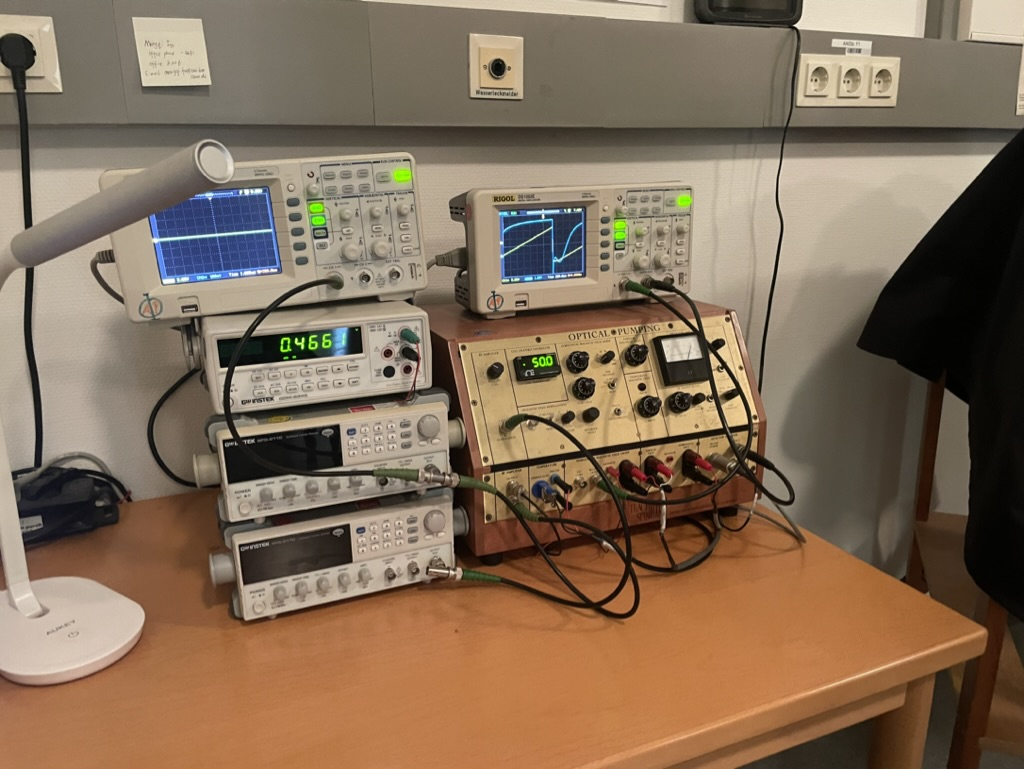
\includegraphics[width=5cm]{Bilddateien/Durchfuehrung/522CFA29-C4DF-4BB6-8FFD-C183A9990129_1_105_c.jpeg}
            \caption{Aufbau der Messgeräte des optischen Pumpens.}
            \label{fig:OptPumpMessgeraete}
        \end{figure}

   
\end{document}